\documentclass[11pt]{article}


\usepackage{amssymb, amsmath, verbatim, amsthm,url, multirow,fullpage,mathtools}
\usepackage{longtable, rotating,makecell,array}
\usepackage[aligntableaux=top]{ytableau}


\setlength{\parindent}{0pt}
\setlength{\parskip}{1.5ex plus 0.5ex minus 0.2ex}


%***************************
%Frontmatter Table of contents
%***************************
% Annotations
%xypic packages
%WLD tkx program
%Useful numeric rings and fields
%Other useful mathematical operations and functions
%Equation display shortcuts
%Shortcuts for frequently used special characters
%Theorem environments
%***************************

%*****************
% Annotations
\usepackage{soul}
\usepackage[colorinlistoftodos,textsize=footnotesize]{todonotes}
\newcommand{\hlfix}[2]{\texthl{#1}\todo{#2}}
\newcommand{\hlnew}[2]{\texthl{#1}\todo[color=green!40]{#2}}
\newcommand{\sanote}{\todo[color=violet!30]}
\newcommand{\note}{\todo[color=green!40]}
\newcommand{\newstart}{\note{The inserted text starts here}}
\newcommand{\newfinish}{\note{The inserted text finishes here}}
\setstcolor{red}
%***************************


%*****************
%xypic packages
\usepackage[all]{xy}
\xyoption{poly}
\xyoption{arc}
%*****************

%*****************
%%% WLD drawing and 2,6 shortcuts

\usetikzlibrary{decorations.pathmorphing,calc}
\usetikzlibrary{intersections}


\definecolor{light-gray}{gray}{0.6}

% some propagator styles
\tikzstyle{propagator}=[decorate,decoration={snake,amplitude=0.8mm}]
\tikzstyle{smallpropagator}=[decorate,decoration={snake,segment length=3mm,amplitude=0.5mm}]

% for highlighting regions of a diagram edge
\tikzstyle{linehighlight}=[red,line width = 3pt,line cap = round, draw opacity = 0.5]

% these two for drawing partial propagators
\tikzstyle{firstdash}=[dashed,line cap=round, dash pattern=on 2pt off 1pt]
\tikzstyle{seconddash}=[dashed,line cap=round, dash pattern=on 0.5pt off 1pt]

% vertices, radius
\newcommand{\drawWLD}[2]{

\pgfmathsetmacro{\n}{#1}
\pgfmathsetmacro{\radius}{#2}
\pgfmathsetmacro{\angle}{360/\n}
\draw (0,0) circle (\radius);
    \foreach \i in {1,2,...,\n} {
      \draw (\angle*\i:\radius) node {$\bullet$};
       %\pgfmathsetmacro{\x}{\angle*\i}
       %\draw[-,shorten >=-\radius*0.1 cm,shorten <=-\radius*0.1 cm]  (\x:\radius cm)-- (\x + \angle: \radius cm);
    }

}

\newcommand{\drawpolypart}[2]{
\pgfmathsetmacro{\n}{#1}
\pgfmathsetmacro{\radius}{#2}
\pgfmathsetmacro{\angle}{360/\n}
    \foreach \i in {1,2,...,\n} {
      \draw (\angle*\i+ \angle/2:\radius) node {$\bullet$};
     \pgfmathsetmacro{\x}{\angle*\i - \angle/2}
      \pgfmathsetmacro{\concave}{((\n-1.5)/\n)}
      \draw (\x:\radius cm) .. controls (\angle *\i: \concave* \radius cm) .. (\x + \angle:\radius cm);
      %\draw (\angle *\i: .8* \radius cm) node {$\bullet$};
    }

}


% r, bumpr, s, bumps: r, s are start/end vertices, bumpr and bumps are how many steps to bump the start/end for multiple props on one edge
\newcommand{\drawprop}[4]{
\pgfmathsetmacro{\r}{#1}
\pgfmathsetmacro{\bumpr}{#2}
\pgfmathsetmacro{\s}{#3}
\pgfmathsetmacro{\bumps}{#4}
\pgfmathsetmacro{\perturbe}{\angle/\n}

\begin{scope}
%\clip (\angle*\r:\radius) -- (\angle + \angle*\r:\radius) -- (\angle*\s:\radius) -- (\angle + \angle*\s:\radius) -- (\angle*\r:\radius);
\draw[smallpropagator] (\angle*\r + \angle/2 + \bumpr*\perturbe:\radius) -- (\angle*\s + \angle/2 + \bumps*\perturbe:\radius);
\end{scope}
}

\newcommand{\drawlabeledprop}[5]{
\pgfmathsetmacro{\r}{#1}
\pgfmathsetmacro{\bumpr}{#2}
\pgfmathsetmacro{\s}{#3}
\pgfmathsetmacro{\bumps}{#4}
\pgfmathsetmacro{\perturbe}{\angle/\n}

\begin{scope}
%\clip (\angle*\r:\radius) -- (\angle + \angle*\r:\radius) -- (\angle*\s:\radius) -- (\angle + \angle*\s:\radius) -- (\angle*\r:\radius);
\draw[smallpropagator] (\angle*\r + \angle/2 + \bumpr*\perturbe:\radius) -- (\angle*\s + \angle/2 + \bumps*\perturbe:\radius) node[midway, below] {#5};
\end{scope}
}


\newcommand{\drawchord}[2]{
\pgfmathsetmacro{\r}{#1}
\pgfmathsetmacro{\s}{#2}

\begin{scope}
%\clip (\angle*\r:\radius) -- (\angle + \angle*\r:\radius) -- (\angle*\s:\radius) -- (\angle + \angle*\s:\radius) -- (\angle*\r:\radius);
\draw (\angle*\r + \angle/2:\radius) -- (\angle*\s + \angle/2:\radius);
\end{scope}
}


% for anything that requires modifying the propagator, e.g. colour, different amplitude,etc
% 5th argument should be {propagator,<other stuff>} or {smallpropagator,<otherstuff>} otherwise you'll get a straight line
\newcommand{\modifiedprop}[5]{
\pgfmathsetmacro{\r}{#1}
\pgfmathsetmacro{\bumpr}{#2}
\pgfmathsetmacro{\s}{#3}
\pgfmathsetmacro{\bumps}{#4}
\pgfmathsetmacro{\perturbe}{\angle/\n}

\begin{scope}
\clip (\angle*\r:\radius) -- (\angle + \angle*\r:\radius) -- (\angle*\s:\radius) -- (\angle + \angle*\s:\radius) -- (\angle*\r:\radius);
\draw[#5] (\angle*\r + \angle/2 + \bumpr*\perturbe:\radius) -- (\angle*\s + \angle/2 + \bumps*\perturbe:\radius);
\end{scope}
}


\newcommand{\boundaryprop}[4]{
\pgfmathsetmacro{\r}{#1}
\pgfmathsetmacro{\bumpr}{#2}
\pgfmathsetmacro{\s}{#3}
\pgfmathsetmacro{\perturbe}{\angle/\n}

\begin{scope}
\clip (\angle*\r:\radius) -- (\angle + \angle*\r:\radius) -- (\angle*\s - \angle:\radius) -- (\angle*\s:\radius) -- (\angle + \angle*\s:\radius) -- (\angle*\r:\radius);
\draw[#4] (\angle*\r + \angle/2 + \bumpr*\perturbe:\radius) -- (\angle*\s:\radius);
\end{scope}
	
}

\newcommand{\drawnumbers}{
  \foreach \i in {1,2,...,\n} {
  \pgfmathsetmacro{\x}{\angle*\i}
  \draw (\x:\radius*1.15) node {\footnotesize \i};
}
}

\newcommand{\drawnumbersshift}{
  \foreach \i in {1,2,...,\n} {
  \pgfmathsetmacro{\x}{\angle*\i + \angle/2}
  \draw (\x:\radius*1.15) node {\footnotesize \i};
}
}



\newcommand{\boundA}[3]{
	\pgfmathsetmacro{\r}{#1}
	\pgfmathsetmacro{\bumpr}{#2}
	\pgfmathsetmacro{\destination}{#3}
	\pgfmathsetmacro{\perturbe}{\angle/\n}
	\path [name path=polyedge1] (\angle*\r:\radius) -- (\angle*\r + \angle:\radius);
	\path [name path=radius1] (0:0) -- (\angle*\r + \angle/2 + \bumpr*\perturbe:\radius);
	\draw[->,
	name intersections={of=polyedge1 and radius1,by=p},
	shorten >=\radius*0.1 cm] (p) ++(\angle*\r + \angle/2 + \bumpr*\perturbe:\radius*0.15) -- (\angle*\destination: \radius*1.15);

}



\newcommand{\boundB}[3]{
	\pgfmathsetmacro{\rangle}{#1*\angle + \angle/2 + #2*\angle/\n}
	\pgfmathsetmacro{\sangle}{#1*\angle + \angle/2 + #3*\angle/\n}


	\draw[->,shorten <=\radius*0.02cm,shorten >=\radius*0.05cm] (\rangle:\radius*1.05) -- (\sangle:\radius*1.05);

}

\newcommand{\makediag}[8]{
	\begin{tikzpicture}[rotate=60,baseline=(current bounding box.east)]
	\begin{scope}
	\drawWLD{6}{0.8}
	%\drawnumbers
	\drawprop{#1}{#2}{#3}{#4}
	\drawprop{#5}{#6}{#7}{#8}
	\end{scope}
	\end{tikzpicture}
}



%%%%%%%
% Drawing partial WLD
%%%%%%%
\def\centerarc[#1](#2)(#3:#4:#5)% Syntax: [draw options] (center) (initial angle:final angle:radius)
    { \draw[#1] ($(#2)+({#5*cos(#3)},{#5*sin(#3)})$) arc (#3:#4:#5); }

\def\clipcenterarc(#1)(#2:#3:#4)% Syntax: [draw options] (center) (initial angle:final angle:radius)
    { \clip ($(#1)+({#4*cos(#2)},{#4*sin(#2)})$) arc (#2:#3:#4); }


%\drawWLDfragment[number of nodes]{radius}{fraction of circle to be displayed}
\newcommand{\drawWLDfragment}[3][10]{
\pgfmathsetmacro{\n}{#1} % use this to get consistent spacing between nodes
\pgfmathsetmacro{\radius}{#2}
\pgfmathsetmacro{\fragment}{#3} % between 0 and 1, gets you that percentage of a circle
\pgfmathsetmacro{\halfangle}{360*\fragment/2}
\pgfmathsetmacro{\startpoint}{270 - \halfangle}
\pgfmathsetmacro{\endpoint}{270 + \halfangle}
\pgfmathsetmacro{\step}{2*\halfangle/\n} 
\pgfmathsetmacro{\zero}{\startpoint-0.5*\step} % so node i is at angle \zero + i*\step
\centerarc[black](0,0)(\startpoint:\endpoint:\radius)
}



\newcommand{\drawnumberspartial}{
\node (0,0) {$\bullet$};
  \foreach \i in {1,2,...,\n} {
  \pgfmathsetmacro{\x}{\step*\i}
  \draw (\zero + \x:\radius*1.15) node {\footnotesize \i};
}
}


\newcommand{\newnode}[3][left]{
	\node[label={[label distance=-1mm]#1:{\scriptsize $#3$}}] at (\zero + #2*\step:\radius) {\scriptsize $\bullet$};
	%\node[#1] at (\zero + #2*\step:\radius) {\scriptsize $#3$};
}

% messier but more flexible: use when you want more control over label placement
\newcommand{\newbetternode}[3][{label distance=-1mm]left}]{
	\node[label={#1:{\scriptsize $#3$}}] at (\zero + #2*\step:\radius) {\scriptsize $\bullet$};
	%\node[#1] at (\zero + #2*\step:\radius) {\scriptsize $#3$};
}



% \newprop[label position]{start node}{end node}{label}
\newcommand{\newprop}[4][midway,below]{
\pgfmathsetmacro{\startnode}{#2}
\pgfmathsetmacro{\endnode}{#3}

\draw[smallpropagator] (\zero+\startnode*\step:\radius) -- (\zero + \endnode*\step:\radius) node[#1] {#4};
}

\newcommand{\newpropbend}[3]{
\draw[smallpropagator] (\zero+#1*\step:\radius*1.1) to[bend left = #3] (\zero + #2*\step:\radius*1.1);
}

%%%%%%%%%%%%%%



%*****************

%*****************
%Useful numeric rings and fields
\newcommand{\Q}{\mathbb{Q}}
\newcommand{\Z}{\mathbb{Z}}
\newcommand{\C}{\mathbb{C}}
\newcommand{\R}{\mathbb{R}}
\newcommand{\N}{\mathbb{N}}
\newcommand{\RP}{\mathbb{R}\mathbb{P}}
\newcommand{\id}{\mathbb{I}}
\newcommand{\Gr}{\mathbb{G}_{\R, \geq 0}}
\newcommand{\Grtnn}{\mathbb{G}_{\R, +}}
\newcommand{\CW}{\overline{\mathcal{W}}} % CW complex of W(k,n)
\newcommand{\BW}{\widehat{\mathcal{W}}} % complex minus bald spots
%*****************


%*****************
%Other useful mathematical operations and functions
\newcommand{\D}{\partial}
\newcommand{\rk}{\textrm{rk }}
\newcommand{\spn}{\textrm{span }}
\newcommand{\rd}{\textrm{d}}
\newcommand{\Res}{\textrm{Res}}
%*****************


%*****************
%Equation display shortcuts
\def\ba #1\ea{\begin{align} #1 \end{align}}
\def\bas #1\eas{\begin{align*} #1 \end{align*}}
\def\bml #1\eml{\begin{multline} #1 \end{multline}}
\def\bmls #1\emls{\begin{multline*} #1 \end{multline*}}
%*****************


%*****************
%Shortcuts for frequently used special characters
\newcommand{\fB}{\mathfrak{B}}
\newcommand{\cP}{\mathcal{P}}
\newcommand{\fZ}{\mathfrak{Z}}
\newcommand{\cM}{\mathcal{M}}
\newcommand{\cA}{\mathcal{A}}
\newcommand{\cI}{\mathcal{I}}
\newcommand{\cC}{\mathcal{C}}
\newcommand{\cB}{\mathcal{B}}
\newcommand{\G}{\mathbb{G}}
\newcommand{\Prop}{\textrm{Prop}}
\newcommand{\cW}{\mathcal{W}}
\newcommand{\bM}{\mathbb{M}}
\newcommand{\cZ}{\mathcal{Z}}
\newcommand{\cY}{\mathcal{Y}}
\newcommand{\Dom}{\textrm{Dom}}
\newcommand{\detzr}[1] {\langle (\cZ_*^\mu|V(p))^{#1} \rangle}
\newcommand{\II}{\mathcal{I}}
\newcommand{\PP}{\mathcal{P}}
\newcommand{\BB}{\mathcal{B}}
\newcommand{\CS}{\mathcal{S}}
\newcommand{\interval}[2]{[\![#1,#2]\!]}
\newcommand{\gale}[1]{\preccurlyeq_{#1}}
\newcommand{\sgale}[1]{\prec_{#1}}
\renewcommand\vec[1]{\overrightarrow{#1}}
\newcommand\cev[1]{\overleftarrow{#1}}
%*****************

%*****************
%Theorem environments
\newtheorem{thm}{Theorem}[section]
\newtheorem{conj}[thm]{Conjecture}
\newtheorem{lem}[thm]{Lemma}
\newtheorem{cor}[thm]{Corollary}
\newtheorem{prop}[thm]{Proposition}
\newtheorem{algorithm}[thm]{Algorithm}


\theoremstyle{remark}
\newtheorem{eg}[thm]{Example}
\newtheorem{claim}[thm]{Claim}

\theoremstyle{definition}
\newtheorem{dfn}[thm]{Definition}
\newtheorem{rmk}[thm]{Remark}
\newtheorem{ntn}[thm]{Notation}
%*****************




\title{Combinatorics of the geometry of Wilson loop diagrams II: Grassmann necklaces, dimensions, and denominators}
\author{Susama Agarwala, Si\^an Fryer, and Karen Yeats}
%\date{}

\begin{document}

\begin{thm}
The Grassmann necklace $(I_1 \ldots I_n)$ from [previous theorem] is the Grassmann necklace for $M(W)$.
\end{thm}

\begin{proof}
We have shown that $(I_1,\dots,I_n)$ is a Grassmann necklace; it remains to check that this Grassmann necklace corresponds to the positroid $M(W)$. Recall from the discussion following Definition~\ref{def:grassmann necklace}, and equation \eqref{basesofmatroids} in particular, that it suffices to show: 
\begin{itemize}
\item For each $i \in [n]$, $I_i$ is a basis for $M(W)$.
\item If $J$ is lexicographically smaller than $I_i$ with respect to $<_i$ (for any $i \in [n]$) then $J$ is not a basis for $M(W)$. 
\end{itemize}
The first point follows immediately: the algorithm is  so $I_i$ is a basis for $M(W)$ by Corollary~\ref{lem basis as perm}.

Now fix $i \in [n]$, and write $I_i = \{a_1 <_i a_2 <_i \dots <_i a_k\}$. This imposes an ordering on the propagators $\cP$, where we label them $p_1, p_2, \dots, p_k$ such that $I_i(p_j) = a_j$ for each $j$. Define $\cP_m: = \{p_1,p_2,\dots,p_m\}$ for each $m\geq 0$, with $\cP_0 = \emptyset$.

We first note that if $a_{m-1}$ and $a_{m}$ are not consecutive vertices for some $m$, then for any intermediate vertex $a_{m-1}<_i x <_i a_{m}$ we must have $\Prop(x) \subseteq \cP_{m-1}$. This is because if any propagator supported on $x$ is still unassigned when the algorithm reaches $x$, we would have $x \in I_i$. We also note that when $p_m$ contributes $I_i(p_m) = a_m$ to the Grassmann necklace, it must be the clockwise-most propagator (amongst those not yet assigned) that is supported on $a_m$ i.e. clockwise-most amongst propagators in the set $\cP \setminus \cP_{m-1}$. 

Now, let $J = \{j_1 <_i j_2<_i \dots <_i j_k\}$ be a $k$-set, and suppose that $J<_i I_i$ in the $<_i$-lexicographic order. Let $m$ be the minimal index such that $j_m <_i a_m$, i.e. the first entry at which $J$ and $I_i$ differ. We will show that $J$ must be a dependent set.

If $\Prop(j_m) = \emptyset$ then $J$ is automatically dependent since the corresponding column of $C(W)$ contains only zeros, so suppose henceforth that $\Prop(j_m) \neq \emptyset$. In particular, this implies that $m>1$, since if $m=1$ we would have $\Prop(j_1) \subseteq \cP_0 = \emptyset$.

In order to exhibit a dependent subset of vertices in $J$, we first define a sequence of sets of propagators by
\[Q_0 = \Prop(j_m), \qquad Q_{l+1} = \Prop(I_i(Q_l))\quad \forall l \geq 0.\]
It is easily verified that this is an increasing chain of sets: indeed, if $q \in Q_l$ then $I_i(q) \in I_i(Q_l)$, and since $I_i(q)$ is one of the vertices that supports $q$ we must have $q \in \Prop(I_i(Q_l)) = Q_{l+1}$. The sequence therefore stabilizes in finitely many steps, since $\cP$ is finite.

We claim that $Q_l \subseteq \cP_{m-1}$ for all $l\geq 0$. The case $l= 0$ follows immediately from the observation above that $\Prop(j_m) \subseteq \cP_{m-1}$. 

Now assume that $Q_0,\dots,Q_{l-1} \subseteq \cP_{m-1}$, and consider $Q_{l}$. If $Q_{l} \setminus Q_{l-1} = \emptyset$ then we are done; if not, let $q \in Q_{l} \setminus Q_{l-1}$. By construction there is some propagator $p_r \in Q_{l-1}$ such that $p_r$ and $q$ are both supported on $I_i(p_r) = a_r$. If $q$ is clockwise of $p_r$ on vertex $a_r$ then we immediately have $q \in \cP_{m-1}$ as observed above. However, if $q$ is counter-clockwise of $p_r$ then we need to show that $p_r$ or another propagator in $Q_l$ constrains the positioning of the other end of $q$ and prevents it from ``escaping'' past $j_m$.

Note that we cannot have $a_r+ 1 = j_m$ when $q$ is counterclockwise of $p_r$, since $q \not\in \Prop(j_m)$ by assumption. If the other end of $p_r$ (i.e. the end not supported on $a_r$) lies on an edge between $a_r$ and $j_m$ then since $q$ is inside $p_r$ with respect to $<_{a_r-1}$ we must have $V(q) \subseteq [a_r-1,j_m]$ and hence $q \in \cP_{m-1}$ by Lemma [no fourth vertex]. In particular, if $l=1$ then $p_r \in Q_{0} = \Prop(j_m)$ and we must be in this case. 

If not, then there must be some propagator $p_s \in Q_{l-2}$ such that $p_r$ and $p_s$ are both supported on $I_i(p_s) := a_s$. Since $p_r$ is clockwise of $q$, and $q$ cannot be supported on $I_i(p_s)$ since $q \not\in Q_{l-1}$, it follows that $I_i(p_s) <_i I_i(p_r)$. Therefore $q$ is inside $p_s$ with respect to $<_{a_s - 1}$ as well.

\begin{figure}[h]
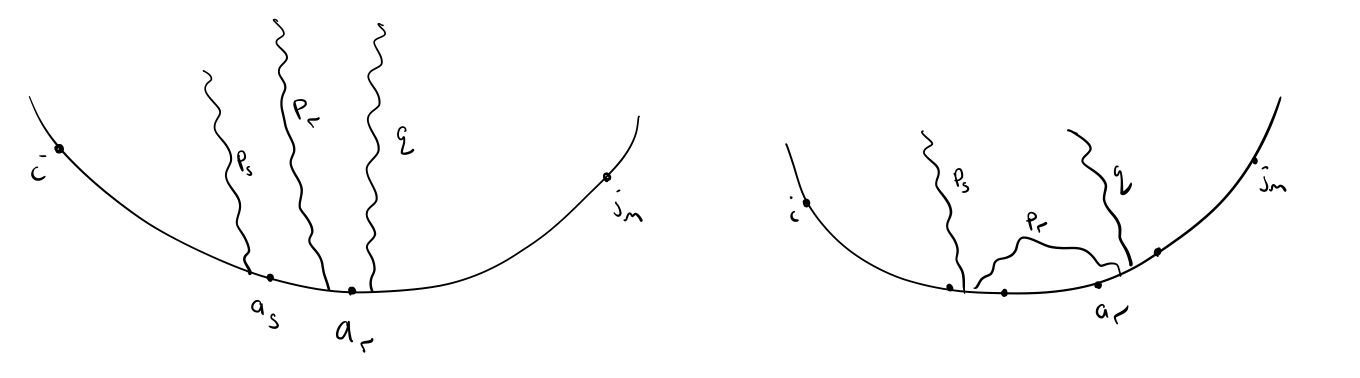
\includegraphics[scale = 0.3]{awkward_induction_case.jpg}
\caption{This picture isn't quite the one we need any more, but it should help to illustrate the claim about $I_i(p_s) <_i I_i(p_r)$}\label{fig:awkward induction step}
\end{figure}

Now repeat the argument above with $p_s$ in place of $p_r$: if the other end of $p_s$ lands on an edge between $q$ and $j_m$ then we have $q \in \cP_{m-1}$ as above; if not then there exists some $p_t \in Q_{l-3}$ with $p_s$ supported on $I_i(p_t)$ and $I_i(p_t) <_i I_i(p_r)$. Since there are finitely many steps this process can take before reaching $Q_0$, and any $p_* \in Q_0  = \Prop(j_m)$ has $j_m$ in its support by definition, this argument eventually terminates with the construction of a propagator constraining the positioning of $q$ as required. This completes the induction step.

Finally, let $Q:= \lim_{l\rightarrow \infty} Q_l$; by the above, this is well-defined and contained in $\cP_{m-1}$. We can now show that $J$ is a dependent set, by constructing a subset $U \subseteq J$ that satifies $|\Prop(U)| < |U|$.

Specifically, we take $U = I_i(Q) \cup \{j_m\}$. This is a subset of $J$ because $I_i$ and $J$ agree on their first $m-1$ terms and $Q \subseteq \cP_{m-1}$. Further, we have $j_m \not\in I_i(Q)$, so $|U| = |I_i(Q)| + 1 = |Q| +1$. On the other hand, since $\Prop(j_m) \subseteq Q$, we have
\[\Prop(U) = \Prop(I_i(Q)) \cup \Prop(j_m) = Q\]
by the construction of $Q$, and hence $|\Prop(U)| = |Q| < |U|$. Thus $J$ is a dependent set, and the Grassmann necklace $(I_1,\dots,I_n)$ constructed from $W$ does indeed define the positroid $M(W)$.
\end{proof}




\end{document}